%!TEX root = ../thesis.tex
%*******************************************************************************
%****************************** X Chapter **********************************
%*******************************************************************************


% **************************** Define Graphics Path **************************
%\ifpdf
%    \graphicspath{{chapter4/figs/raster/}{chapter4/figs/PDF/}{chapter4/figs/}}
%\else
%    \graphicspath{{chapter4/figs/vector/}{chapter4/figs/}}
%\fi
%
\graphicspath{{figs/chapter4/PDF/}}



%%**************************** %Broad Purpose  **********************************
%\section*{Summary and broad purpose of the chapter}
%* How long (number of words)?
%* Deadline
%* What have you got?


\chapter{Nonlinear Dynamics Tools}

\section{Introduction}
The method of state space reconstruction was originally proposed by \cite{packard1980} 
and formalised by \cite{takens1981}. Since then, various investigations and disciplines 
(\cite{aguirre2009, stergiou2011, frank2010, sama2013}) 
relative to nonlinear time series analysis have benefited from it.
The method of state space reconstruction is based on uniform time-delay embedding methodology 
which is a simple matrix implementation that can reconstruct 
an unknown $d-$dimensional manifold $M$ from a scalar time series 
(e.g. one-dimensional time series in $\mathbb{R}$).
A manifold, in this context, is a multidimensional curved surface within a space (e.g. a saddle) 
\cite{guastello-gregson2011}.
Using scalar time series is the main advantage of the method of state space reconstruction 
which in essence preserve dynamic invariants such as correlation dimension, 
fractal dimension, Lyaponov exponents, Kolmogorov-Sinai entropy and detrended 
fluctuation analysis \cite{bradley2015, Quintana-Duque2012, Quintana-Duque2013, 
Quintana-Duque2016, krakovska2015}.
However, selecting appropriate embedding parameters which are necessary to apply 
the state space reconstruction is still an open challenge for which 
we introduce the methodologies to compute such embedding parameters.
In the following subsections, we describe in more detail the state space reconstruction 
theorem (RSSs), uniform time-delay embedding theorem (UTDE),
false nearest neighbours (FNN), average mutual information (AMI) and other 
methodologies for state space reconstruction.




\section{State Space Reconstruction Theorem}
Following the notation employed in \cite{casdagli1991, garland2016, gibson1992,
uzal2011, uzal2010, takens1981}, the method of state space reconstruction is defined by:
%%********************************[EQUATION]************************************
\begin{equation}\label{eq:ssr}
  s(t)=f^t [s(0)],
\end{equation}
%%********************************[EQUATION]************************************
where $s$, $s: A \rightarrow M$ given that $A \subseteq \mathbb{R}$ and $M \subseteq \mathbb{R}^d$,
represents a trajectory which evolves in an unknown $d-$dimensional manifold $M$,
$f: M \rightarrow M$ is an evolution function and $f^t$, with time evolution $t \in \mathbb{N}$,
is the $t$-th iteration of $f$ that corresponds to an initial position $s(0) \in M $ \cite{takens1981}.
Then, a point of a scalar time series $x(t)$ in $\mathbb{R}$, can be obtained with
%%********************************[EQUATION]************************************
\begin{equation}\label{eq:measurement}
  x(t)=h[s(t)],
\end{equation}
%%********************************[EQUATION]************************************
where $h$ is a function, $h: M \rightarrow \mathbb{R}$, defined on the trajectory $s(t)$.

Reconstructed state space can then be described as an $n-$dimensional
 state space defined by $y(t)=\Psi[\boldsymbol{X}(t)]$ where 
$\boldsymbol{X}(t) = \{ x(t), x(t-\tau) , ...,x(t - (m-1)\tau  ) \}$ 
is the uniform time-delay embedding with a dimension embedding $m$
and delay embedding $\tau$ and
$ \Psi: \mathbb{R}^m \rightarrow \mathbb{R}^n$ is a further transformation
of dimensionality (e.g. Principal Component Analysis, Singular Value Decomposition, etc)
being $n \leq m$.
With that in mind, uniform time-delay embedding, $\boldsymbol{X}(t)$, defines a map
$\Phi: M \rightarrow \mathbb{R}^m$ such that $\boldsymbol{X}(t) = \Phi(s(t))$,
where $\Phi$ is a diffeomorphic map \cite{takens1981}
whenever $\tau > 0$ and $m > 2d_{box}$ and $d_{box}$ is the box-counting
dimension of $M$ \cite{garland2016}.
% "Given two manifolds $M$ and $N$, a differientiable map $f: M \rightarrow N$
% is called diffeomorphic if it is one-to-one correspondence and its inverse
% $f^{-1}: N \rightarrow M$ is differientiable as well \cite{wiki:diffeomorphic}".
Then, if $\Phi$ is an embedding of evolving trajectories in the reconstructed space 
then a composition of functions represented with $F^t$ is induced on the
reconstructed state space determined:
%********************************[EQUATION]************************************
\begin{equation}\label{eq:st}
  \boldsymbol{X}(t)=F^t [\boldsymbol{X}(0)] = \Phi \circ f^t \circ \Phi ^{-1}[\boldsymbol{X}(0)].
\end{equation}
%%********************************[EQUATION]************************************
Hence, an embedding is defined as "a smooth
one-to-one coordinate transformation with a smooth inverse" \cite{casdagli1991}.
Figure~\ref{fig:ssr} illustrates the state space reconstruction.
%---------------------------------(FIGURE)-------------------------------------
\begin{figure}
  \centering
    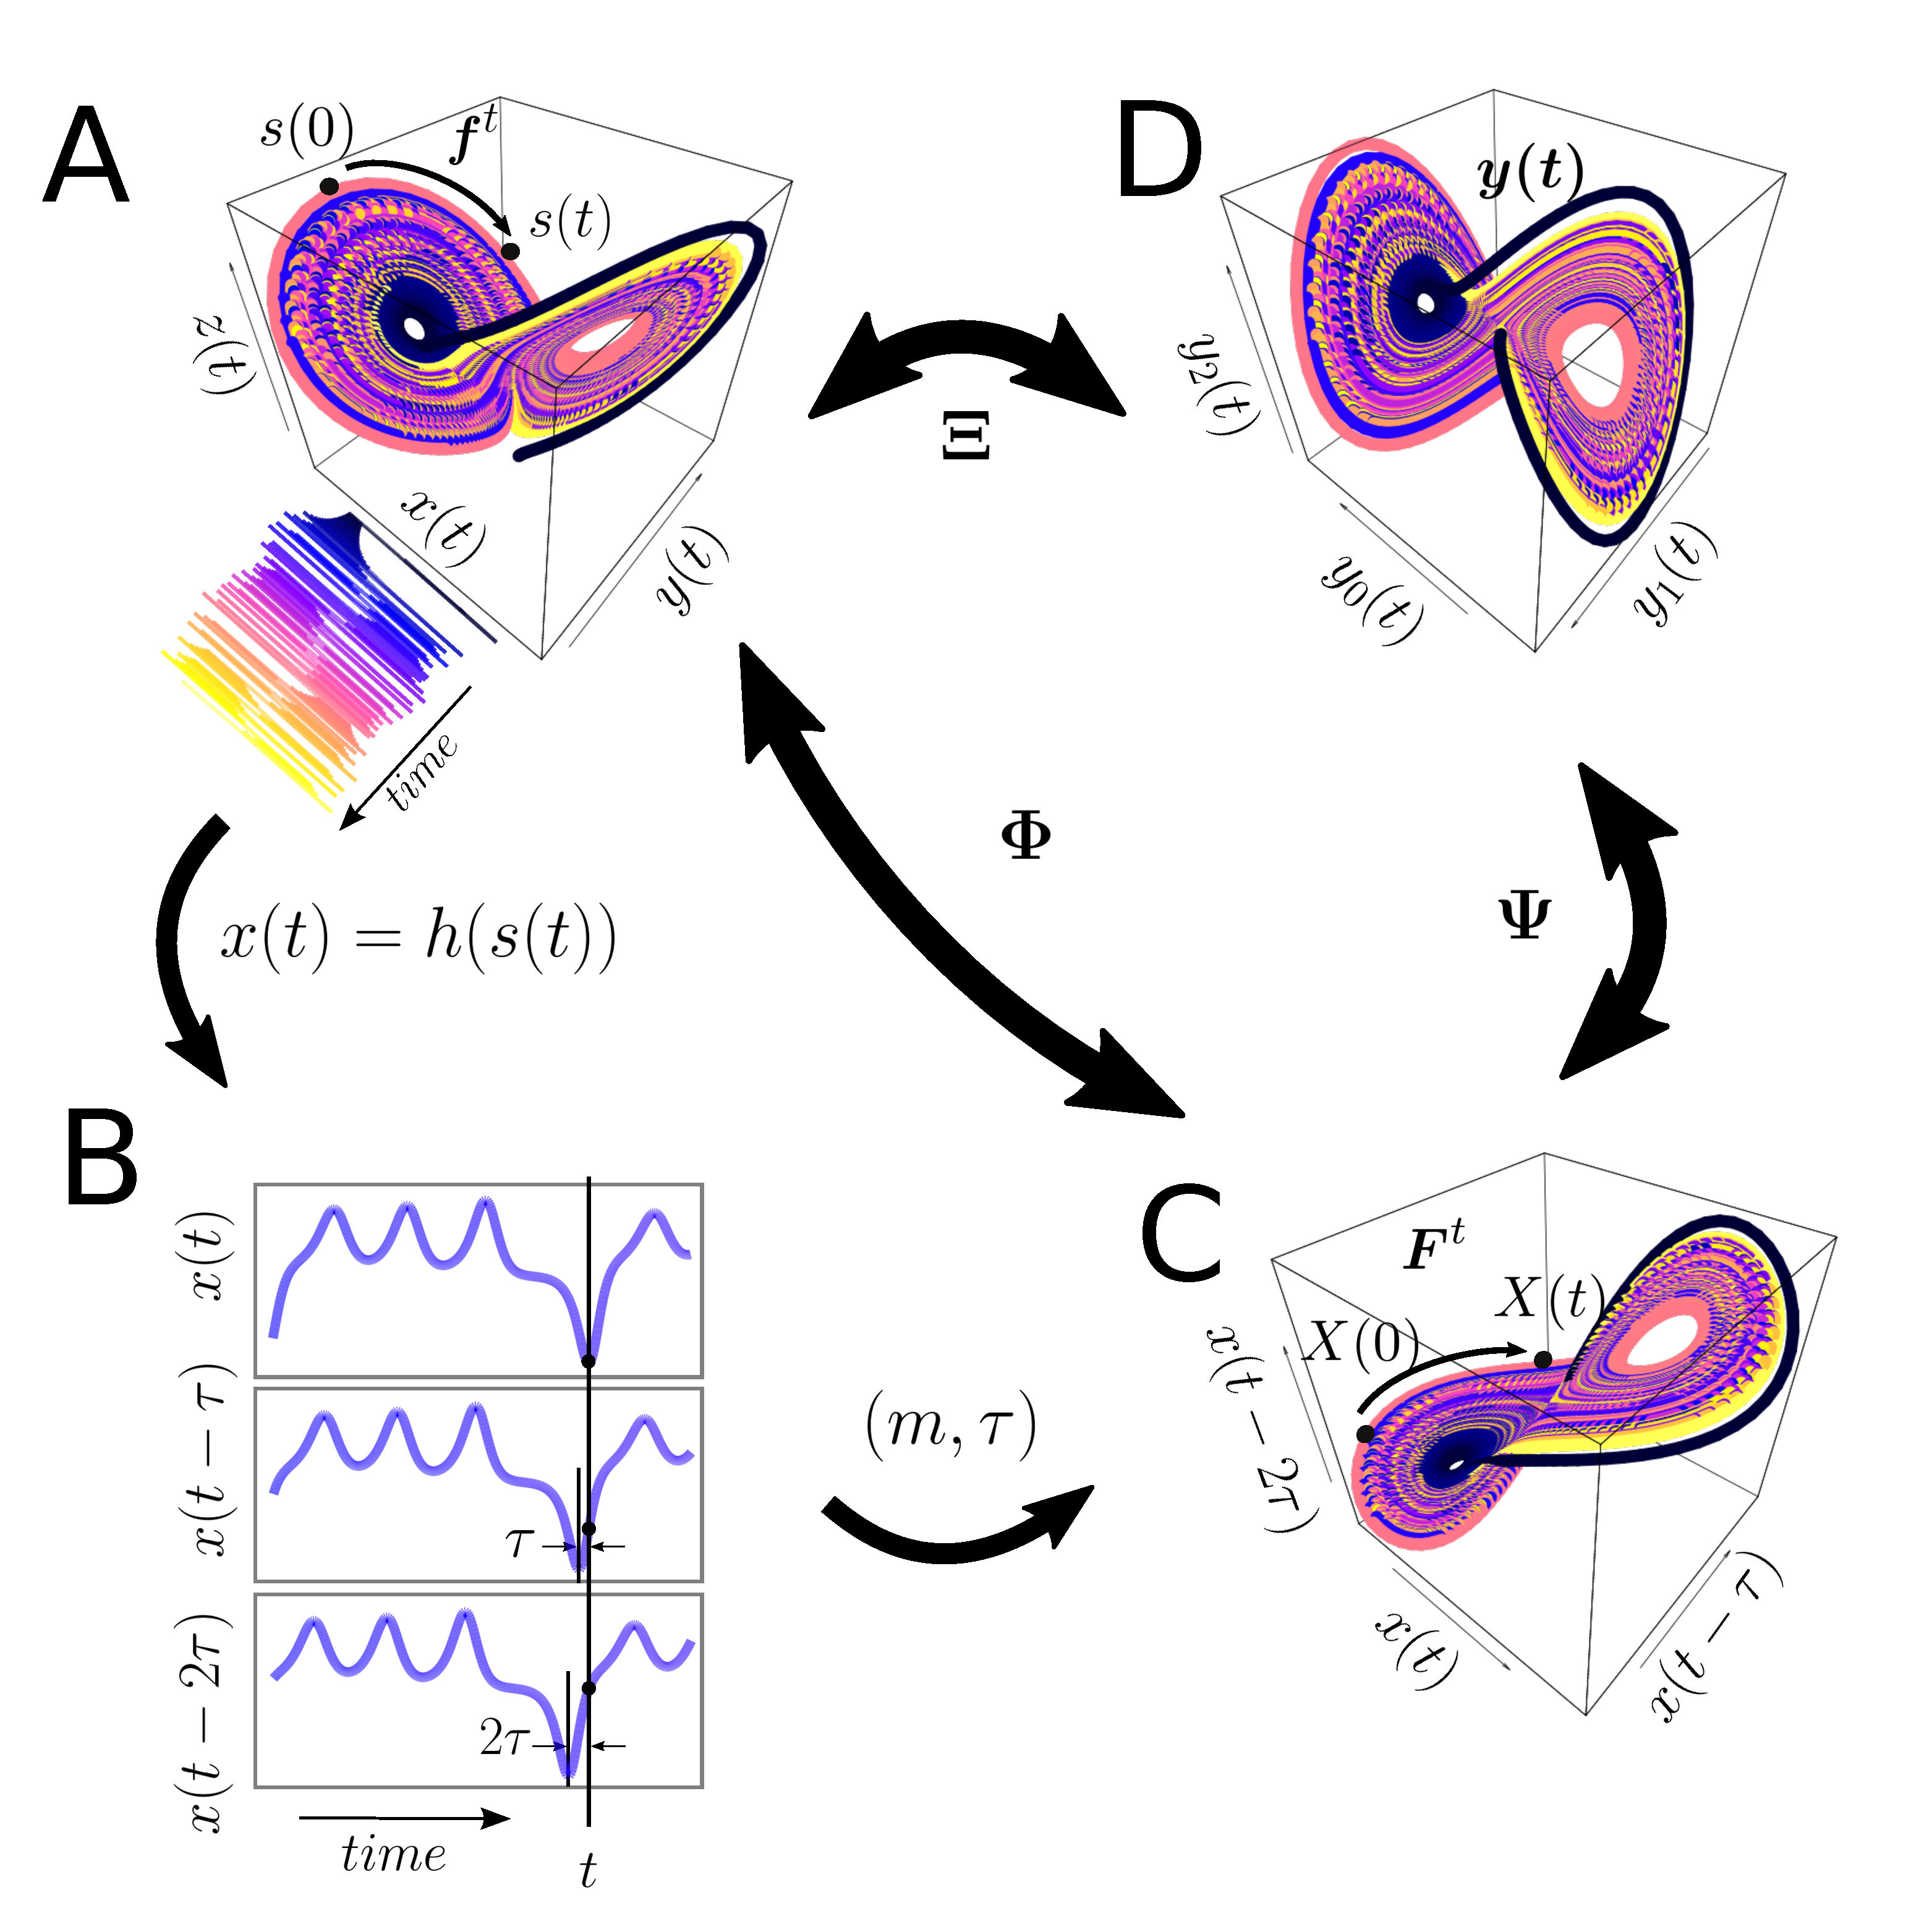
\includegraphics[width=1.0\textwidth]{rss}
    \caption{
	{\bf State space reconstruction methodology.}
	State space reconstruction is based on $x(t)=h[s(t)]= h[f^t [s(0)]]$
	where $h[ ]$ is a function $h: M \rightarrow \mathbb{R}$, defined on the trajectory $s(t)$.
    	$f$ is the true dynamical system, $f:M \rightarrow M$, 
	defined as evolution function and $f^t$, with time evolution $t \in \mathbb{N}$
	which is the $t$-th iteration of $f$ that corresponds to an initial position $s(0) \in M $.
    	The time-delay embedding represented as the $\Phi$, maps the original
    	$d-$dimensional state $s(t)$ into the $m-$dimensional uniform time-delay 
	embedding matrix $\boldsymbol{X}(t)$.
	The transformation map $\Psi$ maps $\boldsymbol{X}(t)$ into a new state $y(t)$ of
	dimensions $n < m$.
	(A) $M-$dimensional state space (e.g. Lorenz system);
    	(B) Delayed copies of $1-$dimensional $x(t)$ from the Lorenz system;
    	(C) $m-$dimensional reconstructed state space with 
	\texorpdfstring{$m$}{m} and    \texorpdfstring{$\tau$}{T}, and 
    	(D) $y(t)$ is the $n-$dimensional reconstructed state space.
	The total reconstruction map is represented as $\Xi = \Psi \circ \Phi $
	where $\Phi$ is the delay reconstruction map and 
	$\Psi$ is the coordinate transformation map.
	This figure is adapted from the work of 
   	\cite{Quintana-Duque2012, casdagli1991, uzal2011}
	and R code to reproduce the figure is available from \cite{hwum2018}.
    }
    \label{fig:ssr}
\end{figure}
%%---------------------------------(FIGURE)-------------------------------------

%%%%%%%%%%%%%%%%%%%%%%%%%%%%%%%%%%%%%%%%%%%%%%%%%%%%%%%%%%%%%%%%%%%%%%%%%%%%%%%%
%%%%%%%%%%%%%%%%%%%%%%%%%%%%%%%%%%%%%%%%%%%%%%%%%%%%%%%%%%%%%%%%%%%%%%%%%%%%%%%%
%%%%%%%%%%%%%%%%%%%%%%%%%%%%%%%%%%%%%%%%%%%%%%%%%%%%%%%%%%%%%%%%%%%%%%%%%%%%%%%%
%%%%%%%%%%%%%%%%%%%%%%%%%%%%%%%%%%%%%%%%%%%%%%%%%%%%%%%%%%%%%%%%%%%%%%%%%%%%%%%%
\section{Uniform Time-Delay Embedding (UTDE)}\label{sec:utimedelayembedding}

\cite{frank2010} and \cite{sama2013} refer to the state space reconstruction method
(\cite{takens1981, casdagli1991}) as "time-delay embeddings" or "delay coordinates", respectively.
However, we consider the term "uniform time-delay embedding"
as more descriptive and appropriate terminology for this thesis.

The uniform time-delay embedding is represented as a matrix of uniform delayed copies 
of the time series $\{ \boldsymbol{x}_n \}_{n=1}^N$ where $N$ is the sample length of
$\{ \boldsymbol{x}_n \}$ and $n$ is index for the samples of $\{ \boldsymbol{x}_n \}$.
$\{ \boldsymbol{x}_n \}_{n=1}^N$ has a sample rate of $T$.
The delayed copies of $\{ \boldsymbol{x}_n \}$ are uniformly separated by $\tau$
and represented as $\{\boldsymbol{ \tilde{x} }_{n- i\tau} \}$
where $i$ goes from $0,1, \dots, (m-1)$ (Fig~\ref{fig:utde}).
$\{\boldsymbol{ \tilde{x} }_{n- i\tau} \}$ contains
information of unobserved state variables and encapsulates the information of
the delayed copies of the available time series in the uniform time-delay embedding matrix 
$\boldsymbol{X}^{m}_{\tau}$, $\boldsymbol{X}^{m}_{\tau} \in \mathbb{R}^m$, defined as
%%********************************[EQUATION]************************************
\begin{equation}\label{eq:tde}
\boldsymbol{X}^{m}_{\tau}  =
\begin{pmatrix}
\boldsymbol{ \tilde{x} }_n \\
\boldsymbol{ \tilde{x} }_{n-\tau} \\
\boldsymbol{ \tilde{x} }_{n-2\tau} \\
\vdots \\
\boldsymbol{ \tilde{x} }_{n- (m-1) \tau} \\
\end{pmatrix}^\intercal, 
\end{equation}
%%********************************[EQUATION]************************************
where $m$ is the embedding dimension, $\tau$ is the embedding delay and
$ ^\intercal$ denotes the transpose.
$m$ and $\tau$ are known as embedding parameters.
%Then after applying the transpose for the vectors of the delayed copies of the time series,
%$\boldsymbol{X}^{m}_{\tau}$, can be represented as
%%********************************[EQUATION]************************************
%\begin{equation}\label{eq:etde2}
%\boldsymbol{X}_{\tau}^{m} =
%\begin{pmatrix}
%  \boldsymbol{X}[ ( (m-1)\tau ) + 1 ] \\
%  \boldsymbol{X}[ ( (m-1)\tau ) + 2 ] \\
%  \vdots \\
%  \boldsymbol{X}[N-1] \\
%  \boldsymbol{X}[N]
%\end{pmatrix}.
%\end{equation}
%%%********************************[EQUATION]************************************
The matrix dimension of $ \boldsymbol{X}_{\tau}^{m} $ is defined by
$N-(m-1)\tau$ rows and $m$ columns and 
$N-(m-1)\tau$ defines the length of each delayed copy 
of $\{ \boldsymbol{ \tilde{x} }_n \}$ in $\boldsymbol{X}^{m}_{\tau}$.
A graphical representation of uniform time-delay embedding is shown in Figure~\ref{fig:utde}.
For further details and explicit examples of uniform time-delay embedding methodology,
we refer the reader to the appendix \ref{appendix:a}.
%---------------------------------(FIGURE)-------------------------------------
\begin{figure}
 \centering
   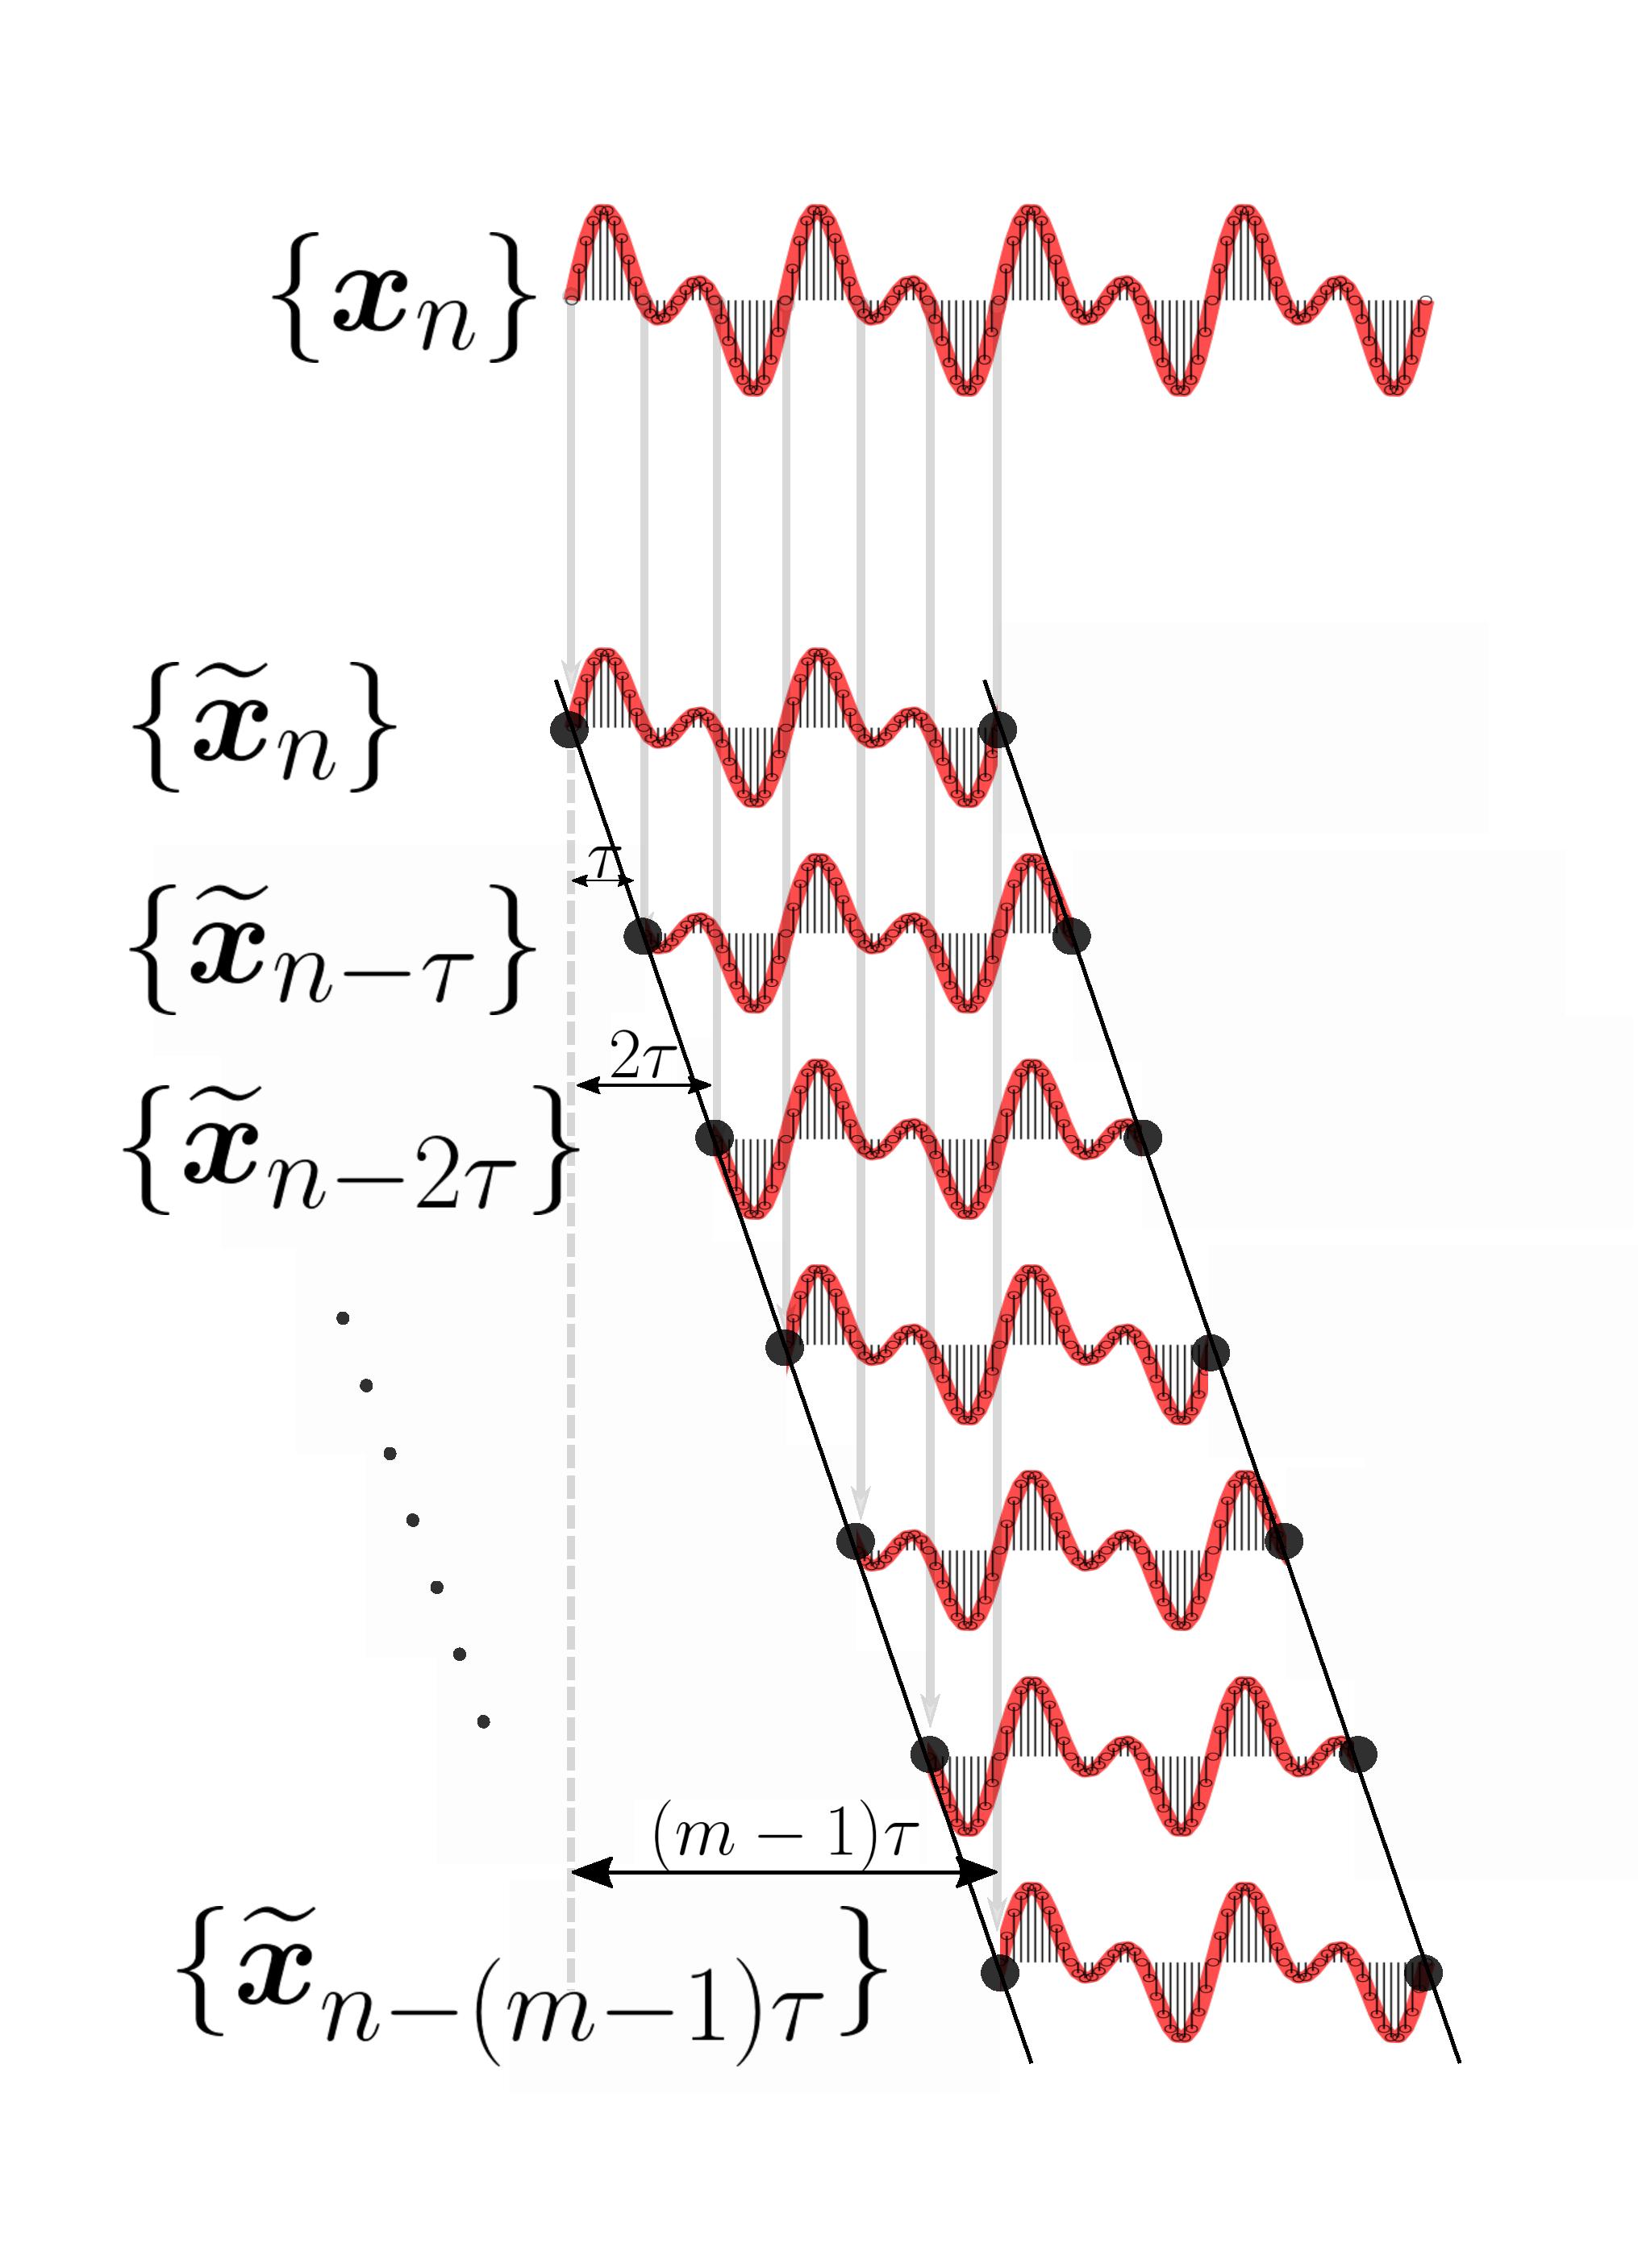
\includegraphics[width=0.95\textwidth]{utde}
   \caption{
	{\bf Uniform time-delay embedding.} 
	UTDE is illustrated as $m-1$ delayed copies
   of $\{ \boldsymbol{x}_n \}$, uniformly separated by $\tau$ and represented as
   $\{ \boldsymbol{ \tilde{x} }_n, \dots,  \boldsymbol{ \tilde{x} }_{n -(m-1)\tau}   \}$ (Eq.~\ref{eq:tde}).
	R code to reproduce figure is available \cite{hwum2018}.
   }
   \label{fig:utde}
\end{figure}
%%---------------------------------(FIGURE)-------------------------------------


%%%%%%%%%%%%%%%%%%%%%%%%%%%%%%%%%%%%%%%%%%%%%%%%%%%%%%%%%%%%%%%%%%%%%%%%%%%%%%%%
%%%%%%%%%%%%%%%%%%%%%%%%%%%%%%%%%%%%%%%%%%%%%%%%%%%%%%%%%%%%%%%%%%%%%%%%%%%%%%%%
%%%%%%%%%%%%%%%%%%%%%%%%%%%%%%%%%%%%%%%%%%%%%%%%%%%%%%%%%%%%%%%%%%%%%%%%%%%%%%%%
%%%%%%%%%%%%%%%%%%%%%%%%%%%%%%%%%%%%%%%%%%%%%%%%%%%%%%%%%%%%%%%%%%%%%%%%%%%%%%%%
\section{Estimation of Embedding Parameters}
The estimation of the embedding parameters ($m$ and $\tau$) 
is a fundamental step for the state space reconstruction with the use
of uniform time-delay embedding method.
Hence, we review two of the most common algorithms,
which will be used in this thesis, to compute the embedding
parameters: the false nearest neighbour (FNN) and the average mutual information (AMI).

%%%%%%%%%%%%%%%%%%%%%%%%%%%%%%%%%%%%%%%%%%%%%%%%%%%%%%%%%%%%%%%%%%%%%%%%%%%%%%%%
%%%%%%%%%%%%%%%%%%%%%%%%%%%%%%%%%%%%%%%%%%%%%%%%%%%%%%%%%%%%%%%%%%%%%%%%%%%%%%%%
%%%%%%%%%%%%%%%%%%%%%%%%%%%%%%%%%%%%%%%%%%%%%%%%%%%%%%%%%%%%%%%%%%%%%%%%%%%%%%%%
%%%%%%%%%%%%%%%%%%%%%%%%%%%%%%%%%%%%%%%%%%%%%%%%%%%%%%%%%%%%%%%%%%%%%%%%%%%%%%%%
\subsection{False Nearest Neighbours}
To select the minimum embedding dimension $m_0$, \cite{kennel1992}
used the method of false neighbours which can be understood as follow:
in one hand, when the embedding dimension is too small to unfold the attractor
"not all points that lie close to each other will be neighbours and some points
appear as neighbours as a result of the attractor being projected down into an
smaller space", on the other hand, when increasing the embedding dimension
 "points that are near to each other in the sufficient
embedding dimension should remain close as the dimension increase from $m$ to $m+1$
\cite{krakovska2015}".
From a mathematical point of view, 
the state space reconstruction theorem is done when the attractor is unfolded with either 
the minimum embedding dimension, $m_0$, or any other embedding dimension value where $m \ge m_0$ \cite{kennel1992}.
On the contrary, any large value of $m_0$ leads to excessive computations \cite{bradley2015}.
Hence, \cite{Cao1997} proposed an algorithm based on the
false neighbour method where only the time-series and one delay embedding value 
are necessary to select the minimum embedding dimension.
Cao's algorithm is based on $E(m)$  which is the mean value of all $a(i,m)$,
both defined as: 
%%********************************[EQUATION]************************************
\begin{equation}\label{eq:e}
  \begin{aligned}
E(m) &= \frac{1}{N-m\tau} \sum_{i=1}^{N-m\tau} a(i,m) \\
    &=
       \frac{1}{N-m\tau} \sum_{i=1}^{N-m\tau}
       \frac{ || \boldsymbol{X}_i(m+1) - \boldsymbol{X}_{n(i,m)}(m+1) || }
            { || \boldsymbol{X}_i(m) - \boldsymbol{X}_{n(i,m)}(m) ||  }
  \end{aligned}
\end{equation}
%%********************************[EQUATION]************************************
where $\boldsymbol{X}_i(m)$ and $\boldsymbol{X}_{n(i,m)}(m)$ are the time-delay
embeddings with $i=1,2,\dots,N-(m-1)\tau$ and $ n(i,m)= 1 \le n(i,m) \le N-m\tau$.
From Eq.~\ref{eq:e} is concluded that $E(m)$ is only dependent on $m$ and $\tau$
for which $E_1(m)$ is defined as
%%********************************[EQUATION]************************************
\begin{equation}\label{eq:e1}
E_1(m) = \frac{ E(m+1) } { E(m)}.
\end{equation}
%%********************************[EQUATION]************************************
$E_1(m)$ is therefore proposed to investigate the variation from $m$ to $m+1$
in order to find the minimum embedding dimension $m_0$ (Eq.~\ref{eq:e1}).
As \cite{Cao1997}, described: "$E_1(m)$ stops changing when $m$ is greater
than some $m_0$, if the time series comes from a multidimensional state space
then $m_0 + 1$ is the minimum dimension".
Additionally, Cao proposed $E_2(m)$ to distinguish deterministic signals from
stochastic signals. $E_2(m)$ is defined as
%%********************************[EQUATION]************************************
\begin{equation}\label{eq:e2}
E_2(m) = \frac{ E^* (m+1) } { E^*(m)},
\end{equation}
%%********************************[EQUATION]************************************
where
%%********************************[EQUATION]************************************
\begin{equation}\label{eq:ee}
E^*(m) = \frac{1}{N-m\tau} \sum_{i=1}^{N-m\tau}
|  \boldsymbol{X}_i(m+1) - \boldsymbol{X}_{n(i,m)}(m+1) |.
\end{equation}
%%********************************[EQUATION]************************************
For instance, when the signal comes from random noise (values that are independent from each other), 
all $E_2(m)$ values are approximately equal to 1 (e.g. $E_2(m) \approx 1$).
However, for deterministic data $E_2(m)$ is not constant for all $m$ (e.g. $E_2(m) \neq 1$).

As an example of the use of $E_1(m)$ and $E_2(m)$ values,
we consider two time series: the solution for the $x$ variable 
of the Lorenz system (Figure~\ref{fig:e1e2}E), and 
a Gaussian noise time series with zero mean and a variance of one 
(Figure~\ref{fig:e1e2}F).
We then compute $E_1(m)$ and $E_2(m)$ values for each time series.
The $E_1(m)$ values for the chaotic time series appear to be constant
after the dimension is equal to six.
The determination of six is given that any value of $m$ can be used as they are within 
the threshold of $1\pm0.05$ (Fig~\ref{fig:e1e2}A).
$E_2(m)$ values, for chaotic time series, are different to one (Fig~\ref{fig:e1e2}C),
for which, it can be concluded that for the chaotic time series the comes 
from a deterministic signal.
With regard to the noise time series,  $E_1(m)$ values appeared to be constant
when $m$ is close to thirteen defined by the same threshold of $1\pm0.05$ (Figure~\ref{fig:e1e2}B) 
and all the $E_2(m)$ values are approximately equal to one (Figure~\ref{fig:e1e2}D). 
$E_1(m)$ values then indicate the minimum embedding dimension of the noisy time series is thirteen,
however all of the $E_2(m)$ values are approximately equal to one (Figure~\ref{fig:e1e2}D)
for which it can be concluded that noise time series
is a stochastic signal.
%%---------------------------------(FIGURE)-------------------------------------
\begin{figure}
  \centering
  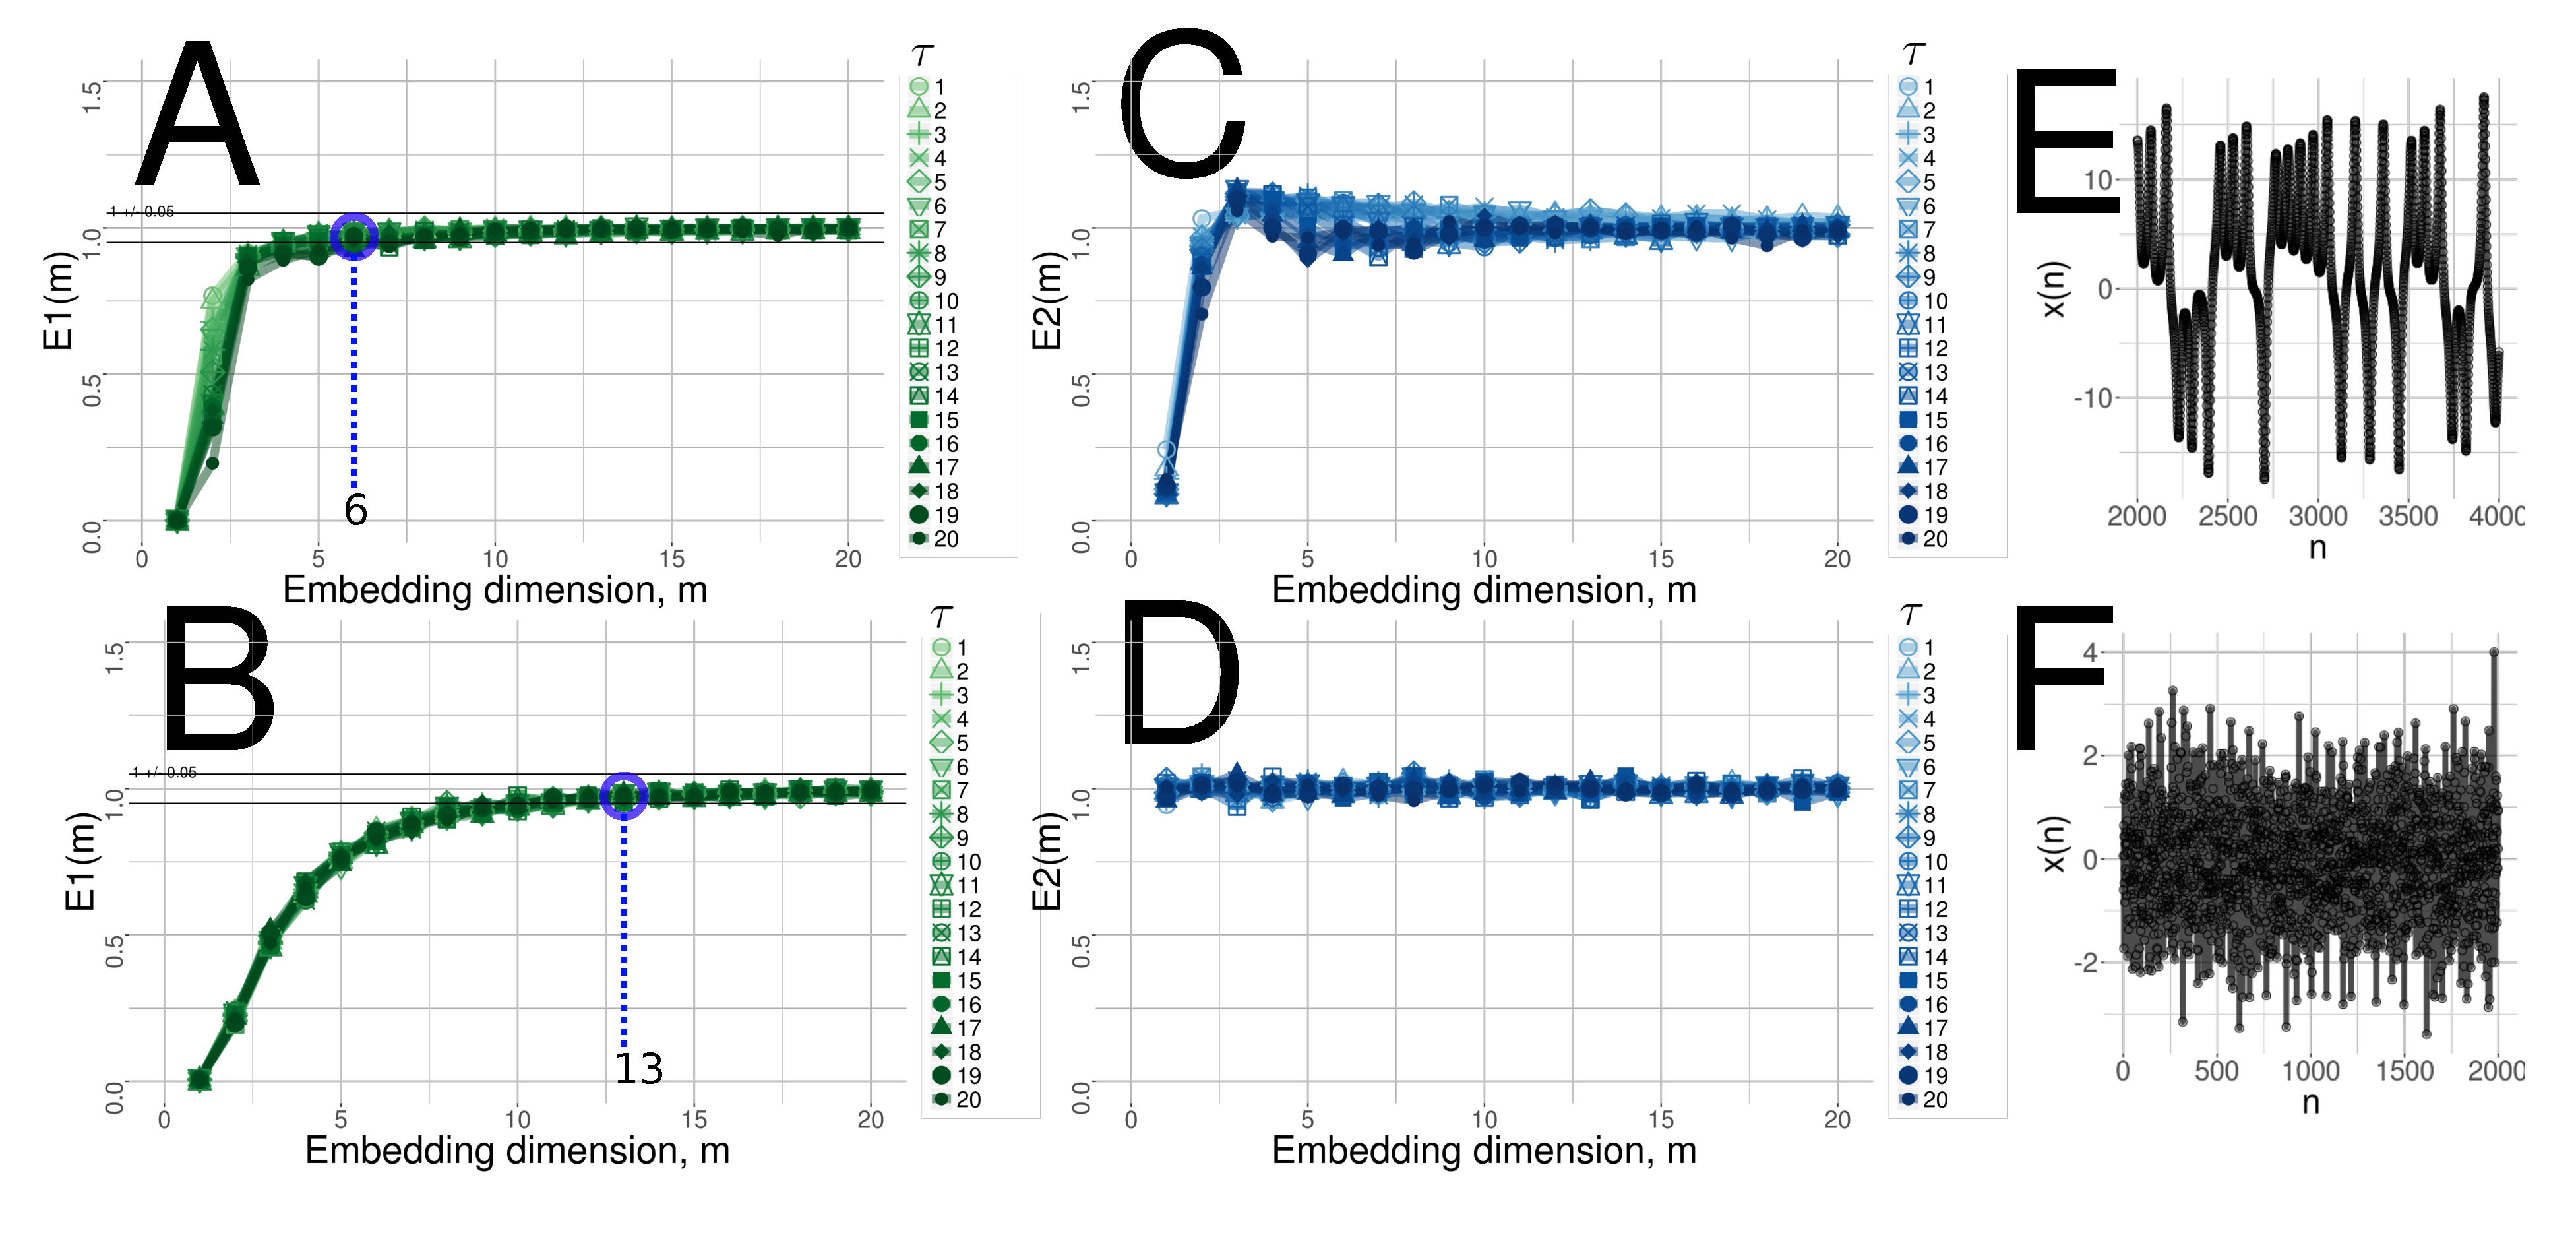
\includegraphics[width=1.0\textwidth]{cao}
    \caption{
	{\bf Minimum dimension embedding values with Cao's method.} 
	(A, B) $E_1 (m)$ values and (C, D) $E_2(m)$ values 
	with variations of $\tau$ values from one to twenty
	for (E) chaotic and (F) random time series.
	R code to reproduce the figure is available from \cite{hwum2018}.
        }
    \label{fig:e1e2}
\end{figure}
%%---------------------------------(FIGURE)-------------------------------------

It is important to note that for this thesis that not only the values for $E_1(m)$ and $E_2(m)$
are computed but also a variation of $\tau$ from 1 to 20 (Figure~\ref{fig:e1e2}A,B,C and D) has been presented.
The purpose of such variation for $\tau$ is to show its independence with
regard to the $E_1(m)$ and $E_2(m)$ values as $\tau$ is increasing (Figure~\ref{fig:e1e2}A,B,C, and D).
However, one negative of the Cao's algorithm \cite{Cao1997} is the definition of 
a new threshold where $m$ values appear to be constant in $E_1 (m)$.
In the case of the given examples and reported results for this thesis, we defined such 
threshold to be 0.05. Further investigation is required for the selection of the threshold 
in the $E_1(m)$, as the selection of the threshold in this work is base on 
no particular method but visual inspection.

Additionally, we observed two negative aspects of the use of the False Nearest 
Neighbour method \cite{Cao1997}: 
(i) the main requirements for the use of Cao's method are the input time series,
a value to set up the maximum embedding dimension and delay embedding, then 
Cao's algorithm compute $E_1(m)$ and $E_2(m)$, however
when the values for $E_1(m)$ stop changing, a threshold should be 
defined in order to obtain the minimum embedding dimension $m_0$, and
(ii) Cao's method compute different estimation of the embedding dimension
when using different window lengths for the time series as shown in chapter 
\ref{chapter6} and \ref{chapter7}.



%%%%%%%%%%%%%%%%%%%%%%%%%%%%%%%%%%%%%%%%%%%%%%%%%%%%%%%%%%%%%%%%%%%%%%%%%%%%%%%
%%%%%%%%%%%%%%%%%%%%%%%%%%%%%%%%%%%%%%%%%%%%%%%%%%%%%%%%%%%%%%%%%%%%%%%%%%%%%%%%
\subsection{Average Mutual Information}
When selecting the delay dimension parameter, $\tau$, 
one can consider the following two cases:
(i) when $\tau$ is too small, the elements of time-delay embedding will be along
the bisectrix of the phase space and the reconstruction is generally not satisfactory, 
(ii) on the contraty, when $\tau$ is too large the elements of the uniform time-delay embedding will
become spread and uncorrelated which makes recovering the underlying
attractor more difficult if not impossible \cite{casdagli1991, emrani2014a, garcia2005e71}.

The autocorrelation function and the average mutual information (AMI) are the
two most commonly used algorithms to compute the minimum delay embedding parameter
$\tau_0$. Similarly, other approaches can be used for the computation of the embedding
parameters \cite{bradley2015}, geometry-based methodologies where the amount of space
filled in the reconstructed state is the metric to compute the delay embedding
\cite{mrosenstein1994} or theoretical approaches to estimate an optimal parameter
for $\tau$ \cite{casdagli1991}. 
\cite{emrani2014a} used the autocorrelation function
in which the first zero crossing is considered as the minimum delay embedding
parameter. However, the autocorrelation function is a linear statistic for
which the AMI is preferred over the autocorrelation
function because the AMI considers the nonlinear dynamical correlations
as discussed in \cite{afraser1986,krakovska2015}.
Hence, the AMI algorithm is described below to estimate the minimum delay 
embedding parameter, \texorpdfstring{$\tau_0$}{T}.


To compute the AMI, an histogram of $x(n)$ using $n$ bins is calculated
and then a probability distribution of data is computed \cite{kantz2003}.
AMI is therefore denoted by $I(\tau)$ which is the average mutual information between
the original time series, $x(n)$, and the delayed time series, $x(n-\tau)$,
delayed by $\tau$ \cite{kabiraj2012}. AMI is defined by
%%********************************[EQUATION]************************************
\begin{equation}\label{eq:ami}
I(\tau) = \sum_{i,j}^N p_{ij} log_2 \frac{ p_{ij} }{ p_i p_j }.
\end{equation}
%%********************************[EQUATION]************************************

Probabilities are defined as follows:
$p_i$ is the probability that $x(n)$ has a value inside the $i$-th bin of the histogram,
$p_j$ is the probability that $x(n+\tau)$ has a value inside the $j$-th bin of the histogram
and let $p_{ij}(\tau)$ be the probability that $x(n)$ is in bin $i$ and $x(n+\tau)$ is in bin $j$.
The AMI is measured in bits (base 2, also called shannons) \cite{kantz2003, nonlinearTseries2016}.
For small $\tau$, AMI will be large and it will then decrease rapidly.
As $\tau$ increase and goes to a large limit, $x(n)$ and $x(n+\tau)$ have nothing
to do with each other and $p_(ij)$ is factorised as $p_ip_j$ for which AMI is close to zero.  
Then, in order to obtain $\tau_0$, "it has to be found in the first minimum of $I(\tau)$ 
where $x(n+\tau)$ adds maximal information to the knowledge from $x(n)$, or,
where the redundancy is the least" \cite{kantz2003}.

For example, we compute the AMI for two time series:
i) the $x$ solution of the Lorenz system, and
ii) a noise time series using a normal distribution with mean zero and standard deviation
equal to one. 
The AMI plots are shown in Figure~\ref{fig:amis}, where 
the minimum delay embedding parameter for the chaotic time series
is $\tau_0=17$ and for the noise time series is  $\tau_0=1$. 
Hence, it can be concluded that the amount of knowledge for any noise time series is zero
for which the first minimum embedding parameter is equal to one. On the
contrary, the first minimum of the AMI for the chaotic time series is $\tau_0=17$
which is the value that maximize the independence in the reconstructed
state space \cite{bradley2015}.
%%---------------------------------(FIGURE)-------------------------------------
\begin{figure}[!h]
  \centering
  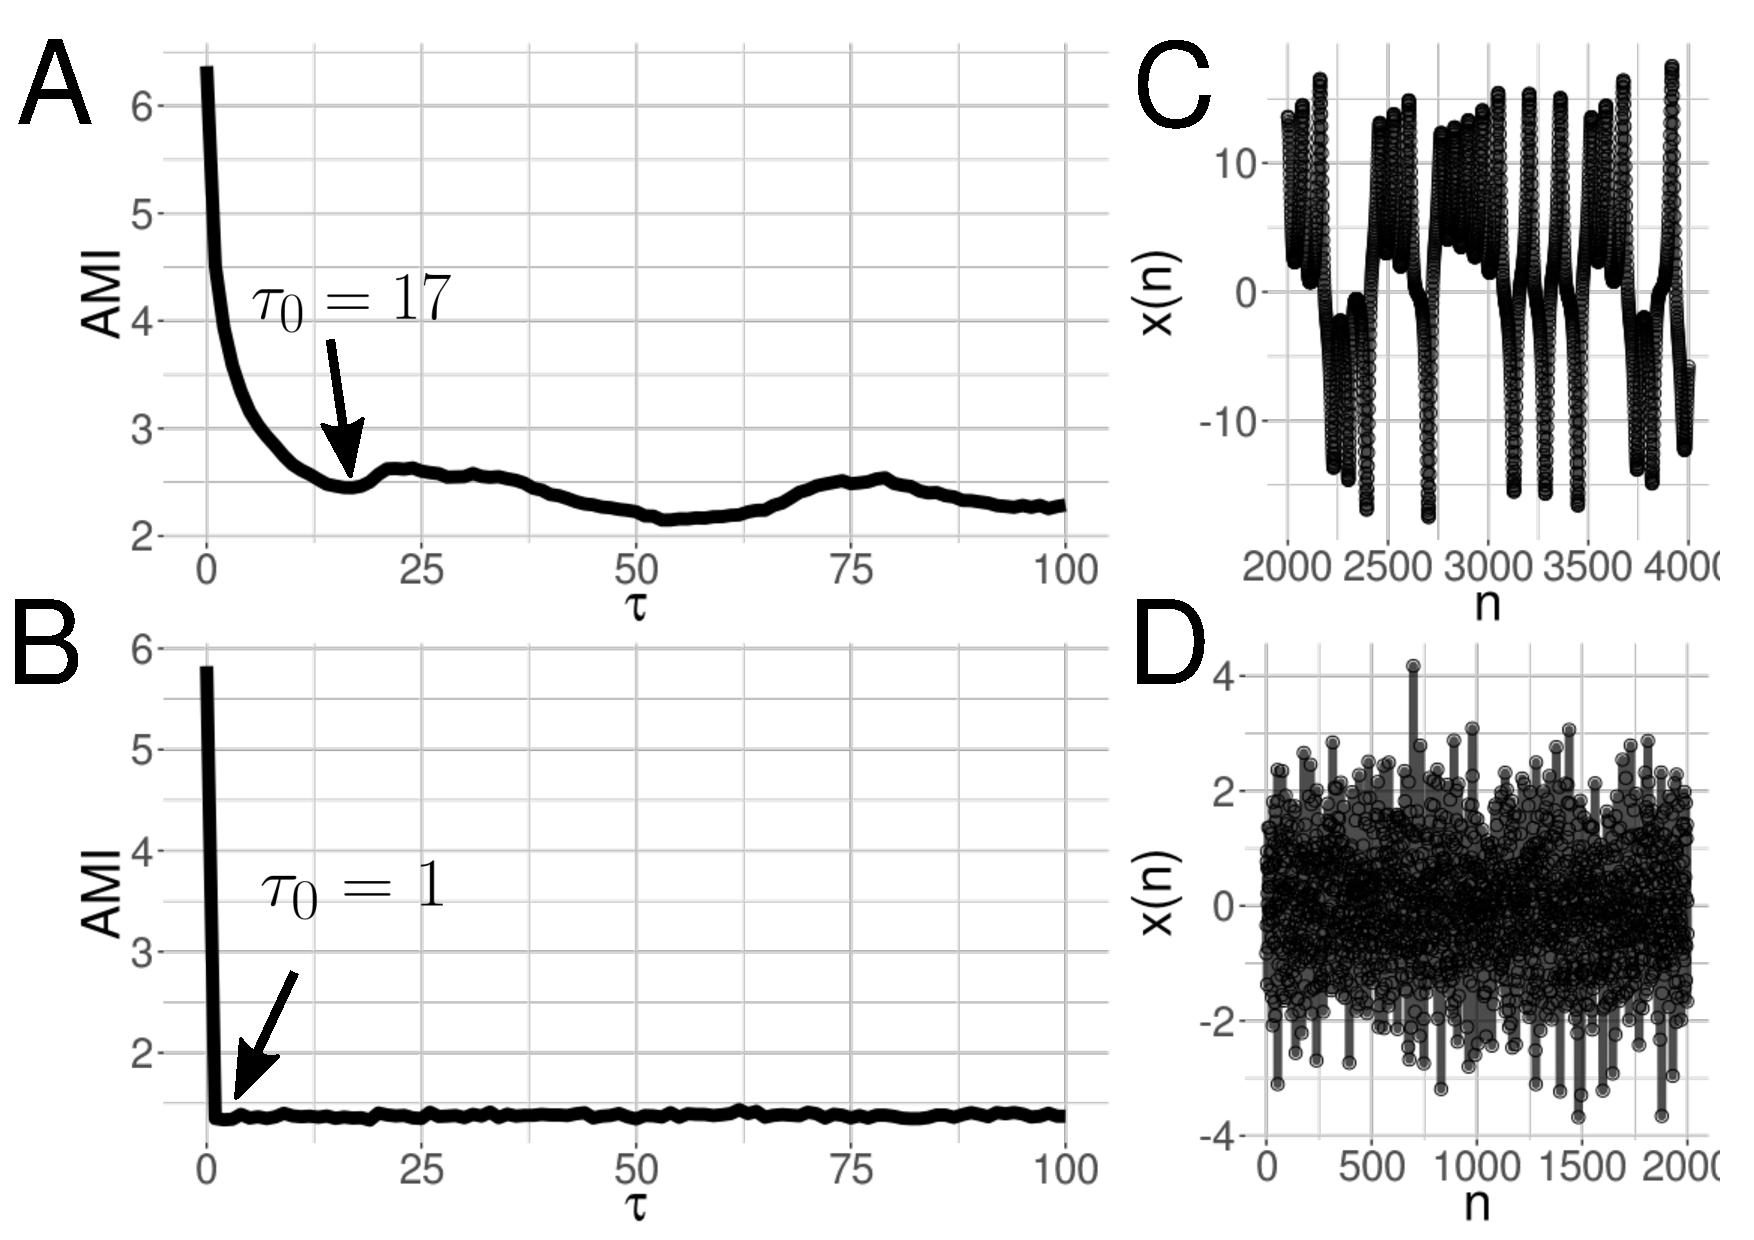
\includegraphics[width=1.0\textwidth]{ami}
    \caption{
	{\bf Minimum delay embedding values with AMI's method.} 
    	(A, B) AMI values where its first minimum value in the curve
	is the minimum time delay embedding ($\tau_0$), 
	for (C) a chaotic and (D) noise time series.
	R code to reproduce the figure is available from \cite{hwum2018}.
        }
    \label{fig:amis}
\end{figure}
%%---------------------------------(FIGURE)-------------------------------------

Similarly as Cao's algorithm negatives, AMI's algorithm is not an
exception for negatives, which are worthwhile to mention for further investigations.
For instance, (i) is not clear why the choose of the first minimum of the AMI is
 the minimum delay embedding parameter \cite{kantz2003} and 
(ii) the probability distribution of the AMI function is computed
with the use of histograms which depends on a heuristic choice of number of bins
for which AMI depends on partitioning \cite{garcia2005e71}, and
(iii) "the method is proposed for two dimensional reconstructions and then 
extended to be used in a multidimensional case which is not necessarily hold in higher dimensions" 
\cite{gomezgarcia2014}.


\subsection{Other methodologies for state space reconstruction.}
In addition to the Uniform Time-Delay Embedding method, 
other methods have recently been investigated to perform state space reconstruction.
For instance, 
(i) the nonuniform time-delay embedding methodology  
where the consecutive delayed copies of $\{ \boldsymbol{x}_n  \} $ are not
equidistant. Such method has been probed to create better representations 
of the dynamics of the state space to analyse, for instance, 
quasiperiodic and multiple time-scale time series over the conventional 
uniform time-delay embedding algorithm 
\cite{pecora2007, uzal2011, Quintana-Duque2012, Quintana-Duque2013, Quintana-Duque2016}, and
(ii) Uniform 2 time-delay embedding method which takes advantage 
of finding an embedding window instead of the traditional method 
of finding the embedding parameters separately \cite{gomezgarcia2014}.
In general, Uniform 2 time-delay embedding method computes $m$ with False Nearest Neighbour (FNN) 
algorithm and $\tau$ is computed as $\tau= d_w / (m-1)$, 
where $d_w$ is given by the minimisation of the Minimum Description Length \cite{small2004}.
However, the previous methods are out of the scope of the thesis
but it is important to refer readers 
to those references for further investigations  in this regard.






\section{Recurrence Plots}

Originally, Henri Poincar\'e in 1890 introduced the concept of recurrences 
in conservative systems, however such discovery was not put into practice 
until the development of faster computers \cite{marwan2007},
for which \cite{eckmann1987} introduced a method
where recurrences in the dynamics of a system can be visualised using Recurrence Plots.
The intention of Eckmann et al. \cite{eckmann1987}  was to propose a tool,
called Recurrence Plot (RP), that provides insights into high-dimensional dynamical 
systems where trajectories are very difficult to visualise.
Hence, "RP is a tool that helps us to investigate the 
$m-$dimensional phase space trajectories through a two-dimensional 
representation of its recurrences" \cite{marwan2015}.
Similarly, Marwan et al. \cite{marwan2015} pointed out that additionally to the methodologies
of the state space reconstruction and other dynamic invariants such as Lyapunov exponent, 
Kolmogorov-Sinai entropy, the recurrences of the trajectories in the phase space 
can provide important clues to characterise natural process that present, for
instance, periodicities (as Milankovitch cycles) or irregular cycles 
(as El Ni\~no Southern Oscillation). 
Such recurrences can not only be visualised using Recurrence Plots (RP) 
but also be quantified with Recurrence Quantification Analysis (RQA) metrics, 
which leads to applications of these tools in various areas such as economy, 
physiology, neuroscience, earth science, astrophysics and engineering \cite{marwan2007}.

For the creation of a recurrence plot based on time series $\{ \boldsymbol{x}_n \}$, 
it is first computed the state space reconstruction 
with uniform time-delay embedding method 
$X(i)=\{ \boldsymbol{ \tilde{x} }_n, \dots,  \boldsymbol{ \tilde{x} }_{n -(m-1)\tau} \}$
where $i=1,\dots,N$, $N$ is the number of considered states of $X(i)$ 
and $X(i) \in \mathbb{R}^m$ \cite{eckmann1987}.
%Then, one plots a black dot at each point $(i,j)$ in the recurrence plot
%for which $X(j)$ is in the ball of radius $\epsilon$ centred at $X(i)$ 
The recurrence plot is therefore a two-dimensional $N \times N$ square matrix, $\mathbf{R}$, 
where a black dot is placed at $(i,j)$ whenever $X(i)$ is sufficiently close to $X(j)$: 
%%********************************[EQUATION]************************************
\begin{equation}
\mathbf{R}^{m}_{i,j} (\epsilon) = \Theta ( \epsilon_i - || X(i) - X(j) ||, \quad X(i) \in \mathbb{R}^m, \quad i,j=1,\dots,N
\end{equation}
%%********************************[EQUATION]************************************
where $N$ is the number of considered states of $X(i)$, $\epsilon$ is a threshold 
distance, $|| \cdotp ||$ a norm, and $\Theta(\cdotp)$ is the Heaviside 
function (i.e. $\Theta(x)=0$, if $x<0$, and $\Theta(x)=1$ otherwise) 
(Fig~\ref{fig:mrp}) \cite{eckmann1987, marwan2007,marwan2015}.
RP is also characterised with a line of identity (LOI) which is a black main 
diagonal line due to $ R_{i,j}=1 (i,j=1,\dots,N)$. 
%%---------------------------------(FIGURE)-------------------------------------
\begin{figure}[!h]
  \centering
    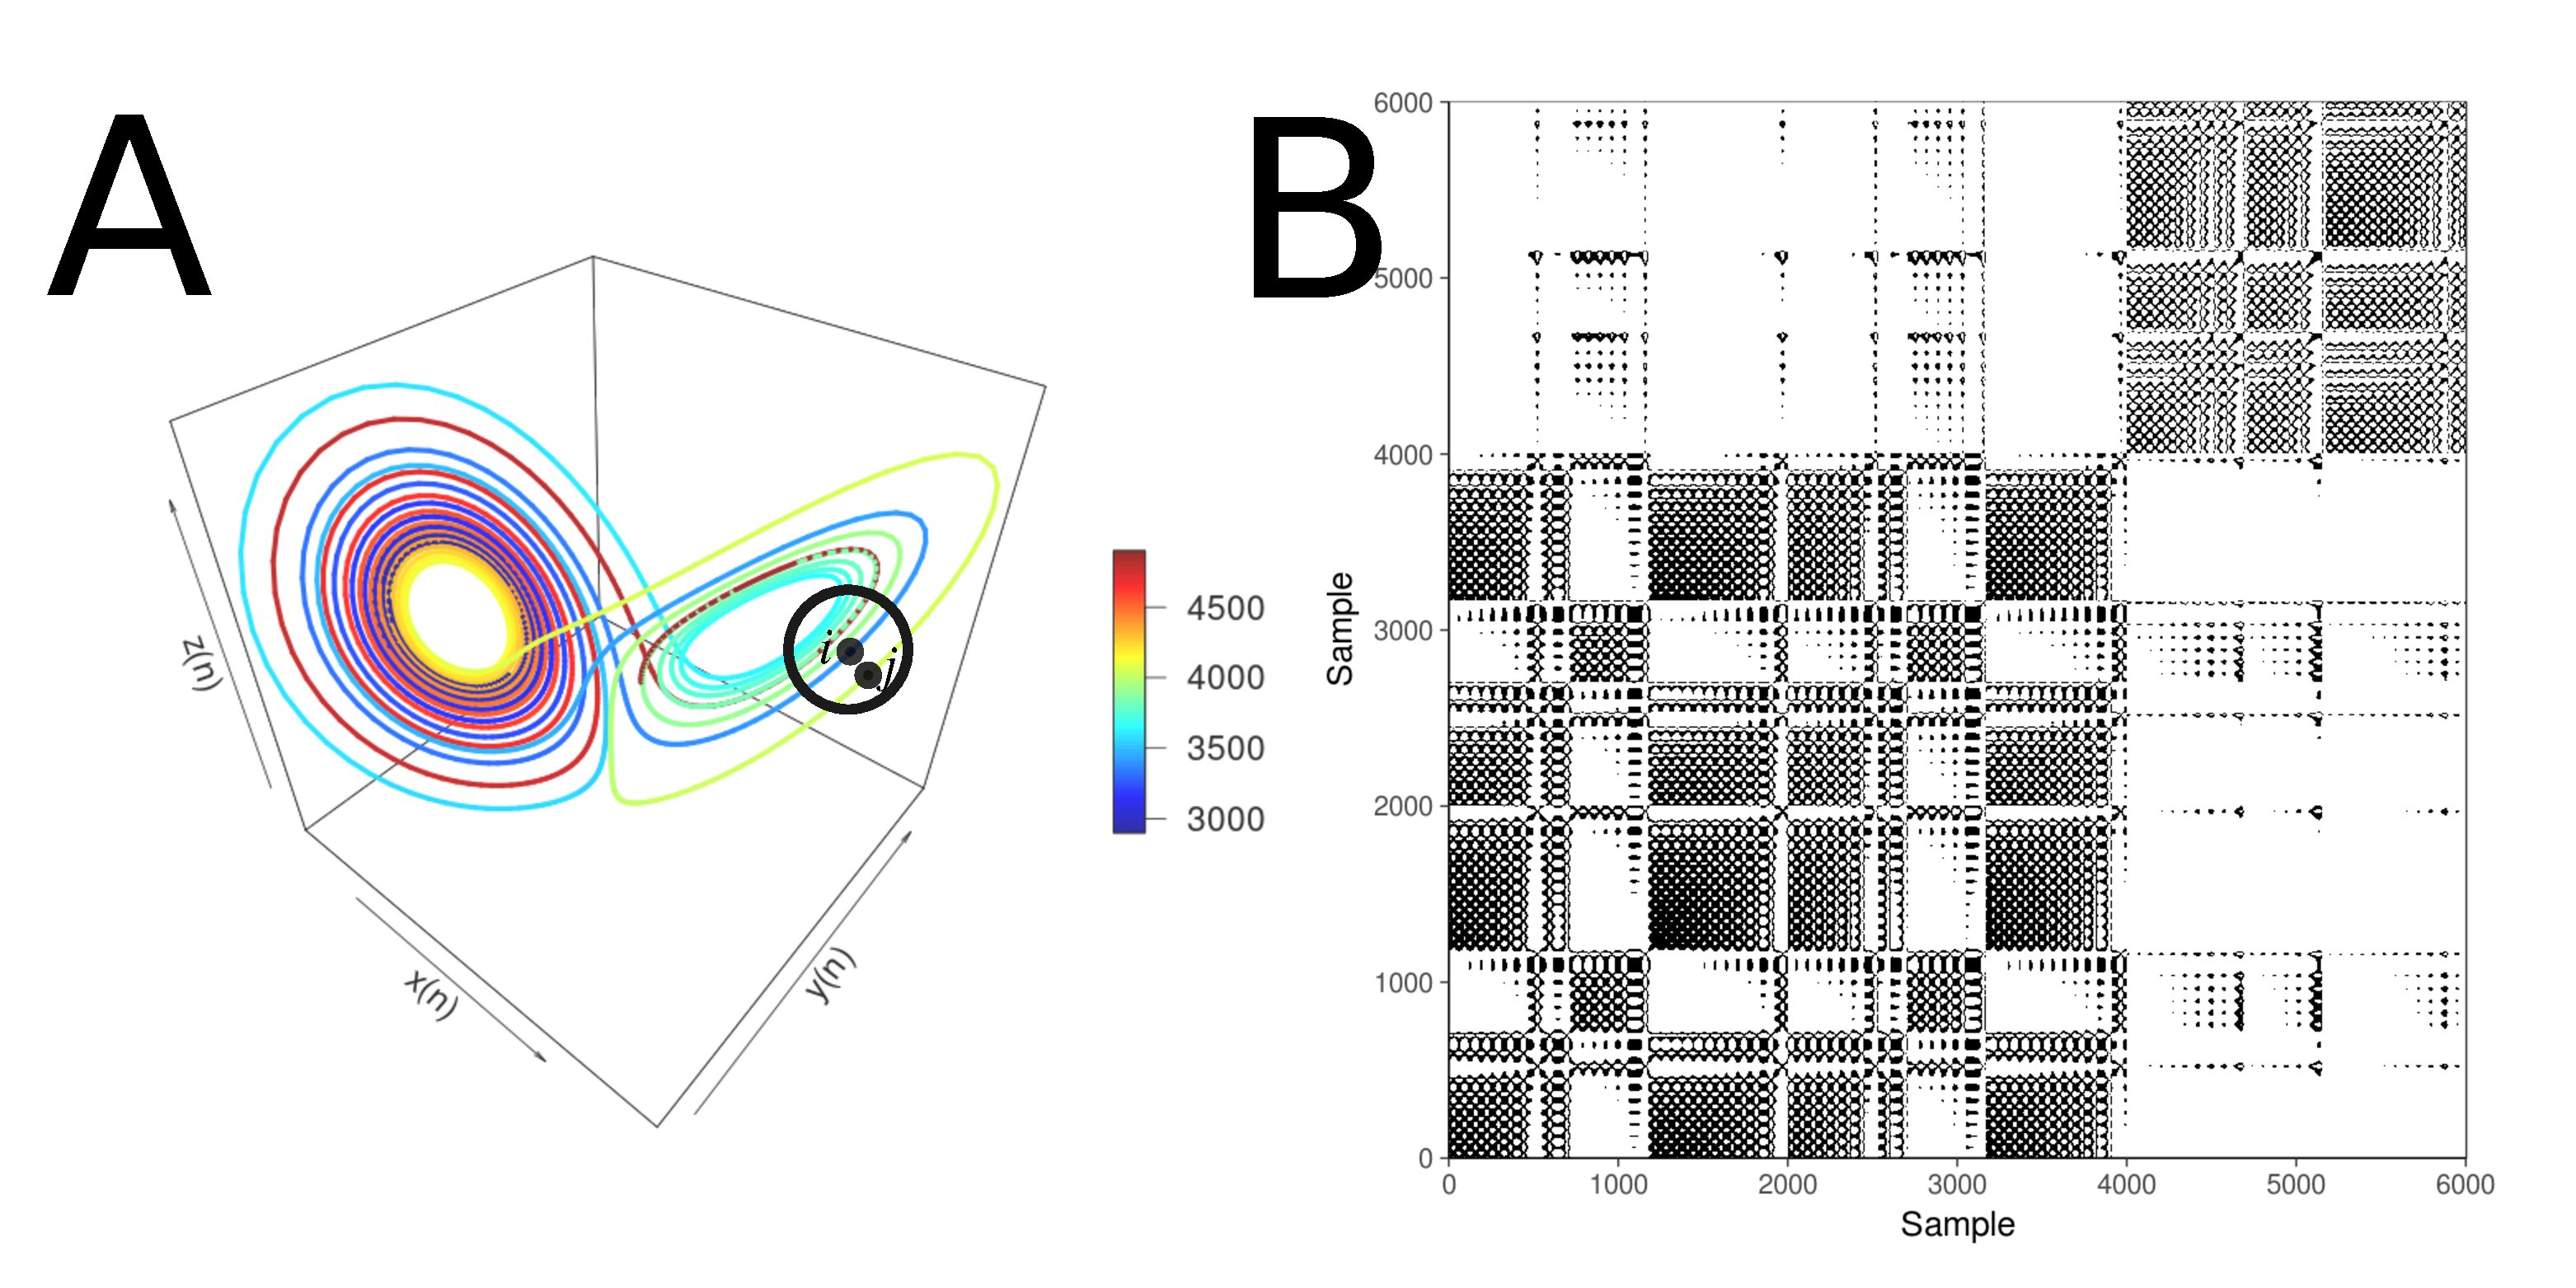
\includegraphics[width=1.0\textwidth]{rp}
    \caption{
	{\bf Recurrence Plots.} 
	(A) State space of the Lorenz system with controlling parameters ($\rho=28, \sigma=10, \beta=8/3$). 
	A point, $j$, in trajectory $X()$ which falls into the neighborhood (black circle) 
	of a given point at $i$ is a recurrent point and is represented as a 
	black dot in the recurrence plot at location $(i, j)$ or white otherwise.
	(B) Recurrence plot using the 
	three components of the Lorenz system and the RP with no embeddings and threshold $\epsilon=5$.
	This figure is adapted from \cite{marwan2015} and R code to reproduce it is available from \cite{hwum2018}.
	}
    \label{fig:mrp}
\end{figure}
%%---------------------------------(FIGURE)-------------------------------------






%%%%%%%%%%%%%%%%%%%%%%%%%%%%%%%%%%%%%%%%%%%%%%%%%%%%%%%%%%%%%%%%%%%%%%%%%%%%%%%%%%%%%%
%%%%%%%%%%%%%%%%%%%%%%%%%%%%%%%%%%%%%%%%%%%%%%%%%%%%%%%%%%%%%%%%%%%%%%%%%%%%%%%%%%%%%%
\section{Structures of Recurrence Plots}

Pattern formations in the RPs can be designated either 
as topology for large-scale patterns or texture for small-scale patterns.
In the case of topology, the following pattern formations are presented:
(i) homogeneous where uniform recurrence points are spread in the RP e.g., 
uniformly distributed noise (Figure~\ref{fig:rp2}A), 
(ii) periodic and quasi-periodic systems where diagonal lines and 
checkerboard structures represent oscillating systems, e.g., sinusoidal signals (Figure~\ref{fig:rp2}B), 
(iii) drift where paling or darkening recurrence points away from 
the LOI is caused by drifting systems, 
e.g., logistic map (Figure~\ref{fig:rp2}C), and
(iv) disrupted where recurrence points are presented white areas or 
bands that indicate abrupt changes in the dynamics, e.g. Brownian motion (Figure~\ref{fig:rp2}D) 
\cite{eckmann1987, marwan2015}.
Texture, for small-scale patterns, can be categorised as:
(i) single or isolated recurrence points that represent rare occurring states, 
do not persist for any time or fluctuate heavily,
(ii) dots forming diagonal lines where the length of the small-scale parallel lines in the diagonal 
are related to the ratio of determinism or predictability in the dynamics of the system, and
(iii) dots forming vertical and horizontal lines where the length of the lines represent 
a time length where a state does not change or change very slowly and the patterns formation 
represent discontinuities in the signal, and
(iv) dots clustering to inscribe rectangular regions which are by related to laminar 
states or singularities \cite{marwan2015}.

%%---------------------------------(FIGURE)-------------------------------------
\begin{figure}
  \centering
    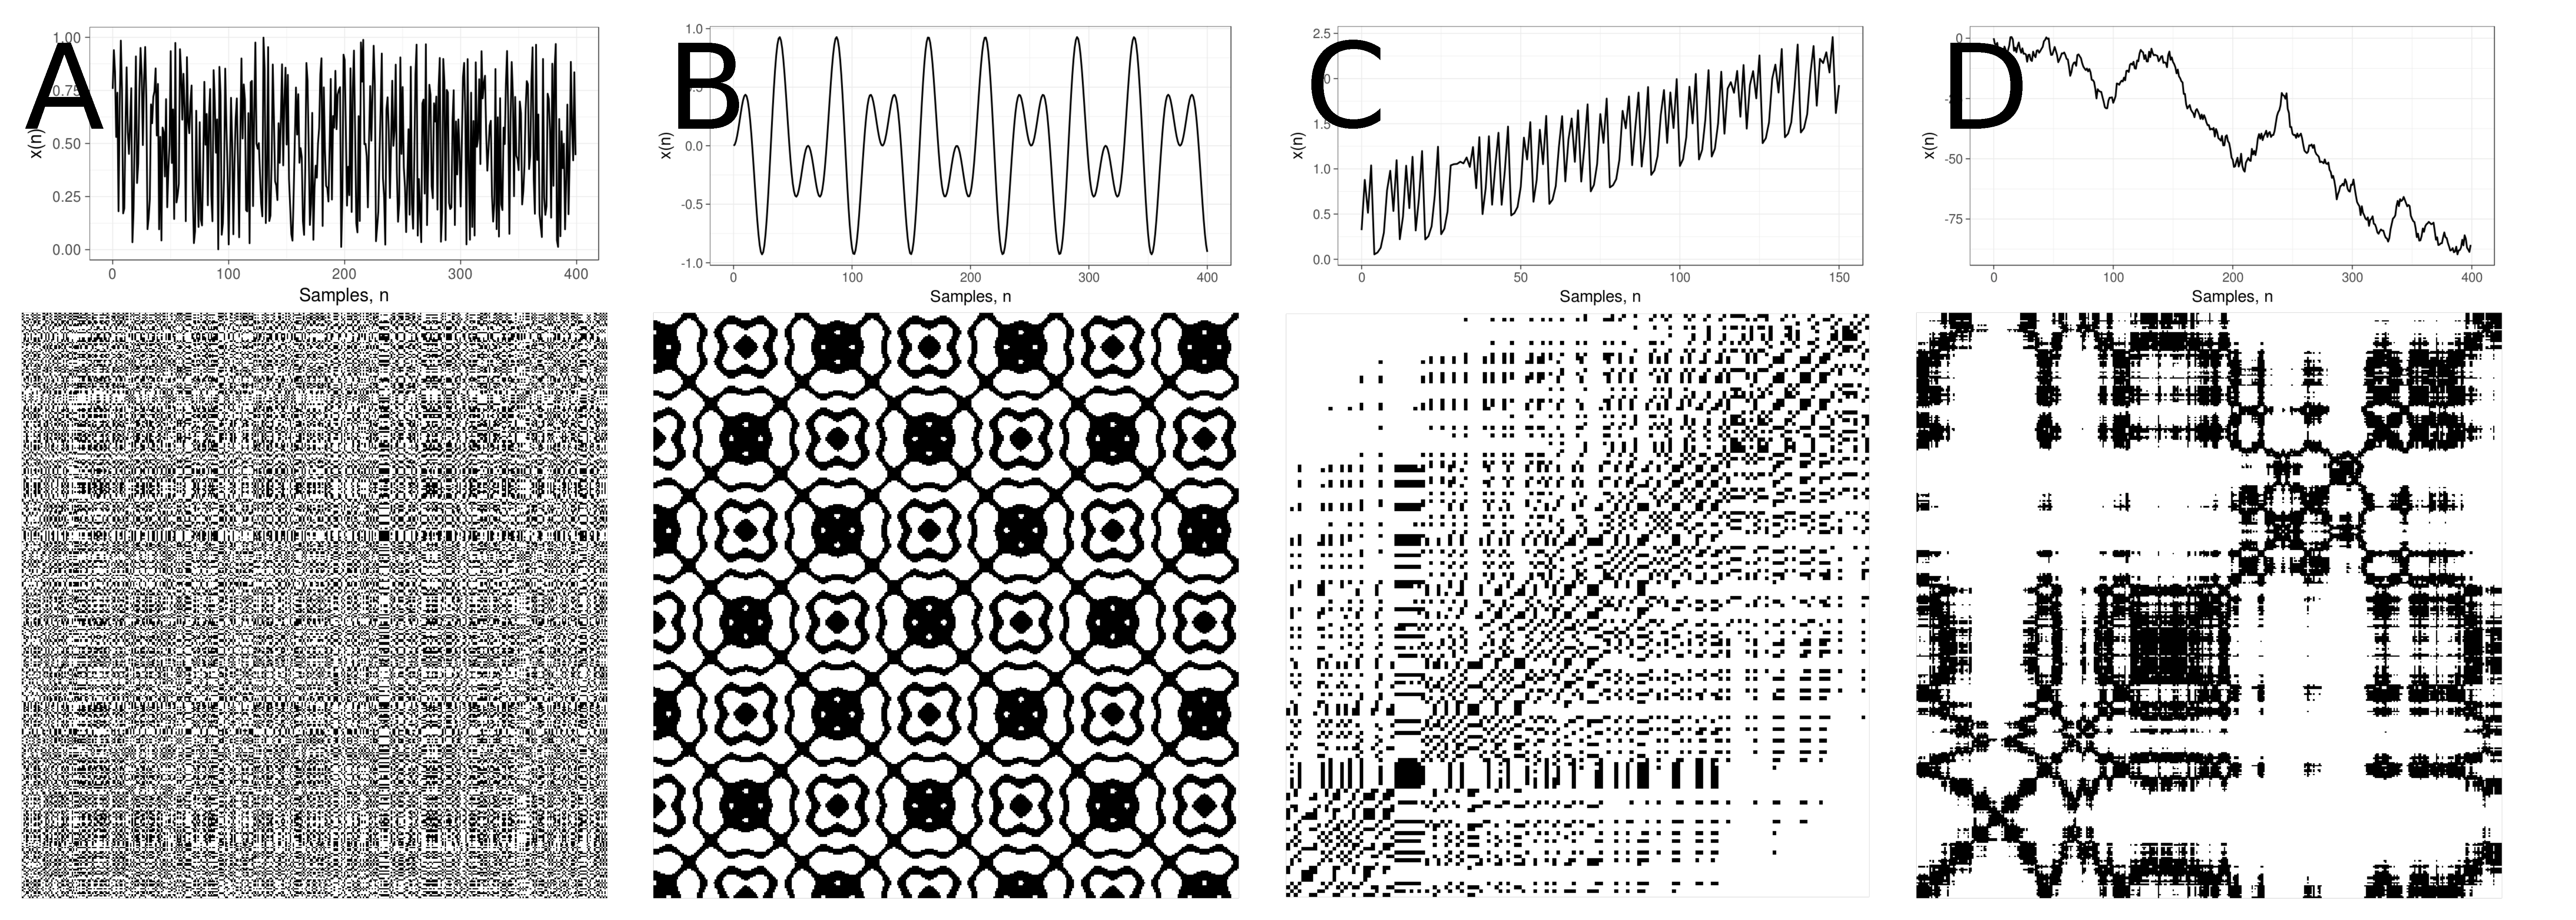
\includegraphics[width=1.0\textwidth]{rpsp}
    \caption{
	{\bf Patterns in Recurrence Plots.} 
	Time-series with its respective recurrence plots for:
	(A) uniformly distributed noise,
	(B) super-positioned harmonic oscillation ($sin( \frac{1}{5}*t) * sin( \frac{5}{100}*t) $),
	(C) drift logistic map ($x_{i+1} = 4 x_i (1- x_i) $) corrupted with a linearly increase term ($0.01*i$), and
	(D) disrupted brownian motion  ($x_{i+1} = x_i + 2*rnorm(1) $).
	Figure is adapted from \cite{marwan2015} and R code to reproduce the figure is available from \cite{hwum2018}.
	}
    \label{fig:rp2}
\end{figure}
%%---------------------------------(FIGURE)-------------------------------------

Although, each of the previous pattern descriptions of the structures in the RP offer 
an idea of the characteristics of dynamical systems from time-series, these descriptions 
might be misinterpreted and conclusions might tend to be subjective as these require 
the interpretation of a researcher(s).
Because of that, recurrence quantification analysis (RQA) offer objective
metrics to quantify the visual characteristics of recurrent 
pattern structures in the RP \cite{zbilut1992}.



%%%%%%%%%%%%%%%%%%%%%%%%%%%%%%%%%%%%%%%%%%%%%%%%%%%%%%%%%%%%%%%%%%%%%%%%%%%%%%%%%%%%%%
%%%%%%%%%%%%%%%%%%%%%%%%%%%%%%%%%%%%%%%%%%%%%%%%%%%%%%%%%%%%%%%%%%%%%%%%%%%%%%%%%%%%%%
\section{Recurrence Quantifications Analysis (RQA)}
Originally, \cite{zbilut1992} proposed metrics to investigate the density of 
recurrence points in RPs, then histograms of lengths for diagonal lines in RPs were 
studied by \cite{trulla1996} which, hence, were the introduction to the term Recurrence 
Quantification Analysis (RQA) by \cite{marwan2008}. 
RQA metrics comprehend percentage of recurrence, percentage of determinism, 
ratio, Shannon entropy of the frequency distributions of the line lengths,
maximal line length and divergence, trend and laminariy \cite{marwan2007, marwan2015}.
%For this work, we considered only four RQA metrics, due to its consistency with our
%preliminary experiments, which are described below.


\subsection{Measures based on the recurrence density}
%%%%%%%%%%%%%%%
%(1st variable) 
The percentage of recurrence (REC) or recurrence rate (RR) is defined as
%%********************************[EQUATION]************************************
\begin{equation}
REC(\epsilon,N)= \frac{1}{N^2 - N} \sum^{N}_{i \neq j = 1} \mathbf{R}^{m}_{i,j}(\epsilon),
\end{equation}
%%********************************[EQUATION]************************************
which enumerates the black dots in the RP excluding the line of identity.
RR is a measure of the relative density of recurrence points in the sparse matrix 
\cite{marwan2015}.
%REC is computed as follow with the nonlinearTseries package \cite{nonlinearTseries} 
%  hist = getHistograms(neighs, ntakens, lmin, vmin)
%  # calculate the number of recurrence points from the recurrence rate. The
%  # recurrence rate counts the number of points at every distance in a concrete
%  # side of the main diagonal.
%  # Thus, sum all points for all distances, multiply by 2 (count both sides) and
%  # add the maindiagonal
%  numberRecurrencePoints = sum(hist$recurrenceHist) + ntakens
%  # calculate the recurrence rate dividing the number of recurrent points at a
%  # given distance by all points that could be at that distance
%  recurrence_rate_vector = hist$recurrenceHist[1:(ntakens - 1)] / ((ntakens - 1):1)
%  # percentage of recurrent points
%  REC = (numberRecurrencePoints) / ntakens ^ 2


\subsection{Measures based on diagonal lines}
%%%%%%%%%%%%%%%
%(2nd variable) 
The percent determinism (DET) is defined as the fraction of recurrence points
that form diagonal lines and it is determined by
%%********************************[EQUATION]************************************
\begin{equation}
DET=\frac{\sum^{N}_{l=d_{min}} l H_D{l} }{\sum^{N}_{i,j=1} \mathbf{R}_{i,j}(\epsilon) },
\end{equation}
%%********************************[EQUATION]************************************
where 
%%********************************[EQUATION]************************************
\begin{equation}
H_D(l) = \sum^{N}_{i,j=1} (1- \mathbf{R}_{i-1,j-1}(\epsilon) ) (1- \mathbf{R}_{i+l,j+l}(\epsilon) ) \prod^{l-1}_{k=0}  \mathbf{R}_{i+k,j+k}(\epsilon)
\end{equation}
%%********************************[EQUATION]************************************
is the histogram of the lengths of the diagonal structures in the RP.
DET can be interpreted as the predictability of the system for periodic signals 
which, in essence, have longer diagonal lines for chaotic signals shorter or 
absent diagonal lines for stochastic signals \cite{marwan2007, marwan2015}.
Similarly, DET is considered as a measurement for 
the organisation of points in RPs  \cite{iwanski1998}. 
%percent determinism (DET) is computed as follow with the nonlinearTseries package \cite{nonlinearTseries}  
% calculateDiagonalParameters = function(ntakens, numberRecurrencePoints,
%                                       lmin = 2, lDiagonalHistogram,
%                                       recurrence_rate_vector, maxDistanceMD) {
%  #begin parameter computations
%  num = sum((lmin:ntakens) * lDiagonalHistogram[lmin:ntakens])
%  DET = num / numberRecurrencePoints


%%%%%%%%%%%%%
%(X variable) 
RATIO is defined as the ratio between DET and REC and it is calculated from 
the frequency distributions of the lengths of the diagonal lines.
RATIO is useful to discover dynamic transitions \cite{marwan2015}.
%  diagP = calculateDiagonalParameters(
%    ntakens, numberRecurrencePoints, lmin, hist$diagonalHist,
%    recurrence_rate_vector, maxDistanceMD
%  )
% calculateDiagonalParameters = function(ntakens, numberRecurrencePoints,
%                                       lmin = 2, lDiagonalHistogram,
%                                       recurrence_rate_vector, maxDistanceMD) {
%  #begin parameter computations
%  num = sum((lmin:ntakens) * lDiagonalHistogram[lmin:ntakens])
%  DET = num / numberRecurrencePoints
% 
%
%    RATIO = diagP$DET / REC
%

%%%%%%%%%%%%%%%%
%(3er variable) 
$D_{max}$ is the longest diagonal line in the RP, defined as
%%********************************[EQUATION]************************************
\begin{equation}
D_{max}= \operatorname*{arg,\max}_{l} H_{D}(l).
\end{equation}
%%********************************[EQUATION]************************************
$D_{max}$ is an indicator of the divergence of trajectory segments.
The smaller $D_{max}$ is, the more divergent the trajectories are \cite{marwan2007, marwan2015}.
According to \cite{iwanski1998}, $D_{max}$ is also related to the inverse 
of the largest positive Lyapunov exponent, where
for example periodic signals tend to have very long lines,
as opposed to the chaotic time series where parallel lines are shorter.
%#'  \item \emph{Lmax}: Length of the longest diagonal line.
%calculateDiagonalParameters = function(ntakens, numberRecurrencePoints,
%                                       lmin = 2, lDiagonalHistogram,
%                                       recurrence_rate_vector, maxDistanceMD) {
%  #pick the penultimate
%  Lmax = tail(which(lDiagonalHistogram > 0), 2)[1]
%  if (is.na(Lmax) || Lmax == ntakens) {
%    Lmax = 0
%  }
  

%%%%%%%%%%%%%%
%(X variable) 
The average diagonal line length is defined as
%%********************************[EQUATION]************************************
\begin{equation}  
\langle D \rangle = \frac{ \sum^{N}_{l=d_{min}} l H_D(l) }{ \sum^{N}_{l=d_{min}}  H_D(l)},
\end{equation}
%%********************************[EQUATION]************************************
and it is the average time that two segments of the trajectory are close to each other.
$\langle D \rangle$ can be interpreted as a measure for determinism (predictability) of the 
system \cite{marwan2007, marwan2015}.
%#'  \item \emph{Lmean}: Mean length of the diagonal lines. The main diagonal is
%#'   not taken into account.
%
% calculateDiagonalParameters = function(ntakens, numberRecurrencePoints,
%                                        lmin = 2, lDiagonalHistogram,
%                                       recurrence_rate_vector, maxDistanceMD) {
%  DET = num / numberRecurrencePoints
%  Lmean = num / sum(lDiagonalHistogram[lmin:ntakens])
%  aux.index = lmin:(ntakens - 1)
%  LmeanWithoutMain = (
%    sum((aux.index) * lDiagonalHistogram[aux.index]) /
%      sum(lDiagonalHistogram[aux.index])
%  )
  


%%%%%%%%%%%%%%%
%(4th variable) 
ENT is the Shannon entropy of the frequency distribution of the diagonal line lengths and
it is defined as
%%********************************[EQUATION]************************************
\begin{equation}
ENT= - \sum^{N}_{l=d_{min}} p(l) ln p(l) \quad with \quad p(l)=\frac{ H_D(l) }{ \sum^{N}_{ l=d_{min} } H_D(l) }.
\end{equation}
%%********************************[EQUATION]************************************
ENT reflects the complexity of the deterministic structure in the system.
For instance, for uncorrelated noise or oscillations, 
the value of ENT is rather small and indicates low complexity of the system,
therefore "the higher the ENT is the more complex the dynamics are" \cite{marwan2007, marwan2015}.
%#'  \item \emph{ENTR}: Shannon entropy of the diagonal line lengths distribution
%
%calculateDiagonalParameters = function(ntakens, numberRecurrencePoints,
%                                       lmin = 2, lDiagonalHistogram,
%                                       recurrence_rate_vector, maxDistanceMD) {
%
%  pl = lDiagonalHistogram / sum(lDiagonalHistogram)
%  diff_0 = which(pl > 0)
%  ENTR = -sum(pl[diff_0] * log(pl[diff_0]))

 

%(5th variable) 
Trend (TND) "is a linear regression coefficient over the
recurrence point density of the diagonals parallel to the LOI" \cite{marwan2015} 
and is defined as
%%********************************[EQUATION]************************************
\begin{equation}
TND= \frac{ \sum^{\tilde{N} }_{i=1}  (1- \tilde{N} /2 )( RR_i - \langle RR_i  \rangle )  }{  \sum^{\tilde{N} }_{i=1}  (i-\tilde{N} /2)^2  }.
\end{equation}
%%********************************[EQUATION]************************************
Trend value "provides information about the stationarity versus nonstationarity 
in the process" \cite{marwan2015}.
TNT values near to zero represent quasi-stationary dynamics and TNT values far from zero
represent nonstationary dynamics that reveal the "drift in the dynamics" \cite{marwan2015}.
TNT measures how quickly the RP pales away from the main diagonal \cite{iwanski1998}.
%#'  \item \emph{TREND}: Trend of the number of recurrent points depending on the
%#'   distance to the main diagonal
%calculateDiagonalParameters = function(ntakens, numberRecurrencePoints,
%                                       lmin = 2, lDiagonalHistogram,
%                                       recurrence_rate_vector, maxDistanceMD) {
%  
%  # use only recurrent points with a distance to the main diagonal < maxDistance
%  recurrence_rate_vector = recurrence_rate_vector[1:maxDistanceMD]
%  mrrv = mean(recurrence_rate_vector)
%  #auxiliar vector for the linear regresion: It is related to the general regression
%  #formula xi-mean(x)
%  auxiliarVector = (1:maxDistanceMD - (maxDistanceMD + 1) / 2)
%  auxiliarVector2 = auxiliarVector * auxiliarVector
%  # divide by two because we are having into account just one side of the main diag
%  num = sum(auxiliarVector * ((recurrence_rate_vector - mrrv) / 2))
%  den = sum(auxiliarVector2)
%  TREND = num / den


\subsection{Measures based on vertical lines}
The previous RQA metrics are based on length, number and distribution of diagonal lines. 
However, patterns for horizontal and vertical lines 
can also be quantified. The following are some examples.

%%%%%%%%%%%%%%%
%(6th variable)
Laminarity (LAM) computes the percentage of recurrence points in vertical lines
which is analogous to the DET variable \cite{marwan2015}.
%#'  \item \emph{LAM}: Percentage of recurrent points that form vertical lines.
%calculateVerticalParameters = function(ntakens, numberRecurrencePoints,
%                                       vmin = 2, verticalLinesHistogram) {
%  #begin parameter computations
%  num = sum((vmin:ntakens) * verticalLinesHistogram[vmin:ntakens])
%  LAM = num / numberRecurrencePoints
 
%%%%%%%%%%%%%%%%
%(7th variable) 
Trapping time (TT) variable computes the average length of vertical lines. 
"TT contains information about the amount and length of vertical 
structures in the RP" which represent 
"the mean time the system will" stay "at a specific time" \cite{marwan2015}.

%%%%%%%%%%%%%%%
%(8th variable) 
The maximal length of the vertical structures $V_{max}$ represents 
"the longest vertical line in the RP" which is analogous to $D_{max}$. 
According to Marwan et al. \cite{marwan2015} the dynamical interpretation 
of this variable is not clear but only as a relationship with 
"singular states in which the system is stuck in a holding pattern
inscribing rectangles in the RP".
%#'  \item \emph{Vmax}: Longest vertical line.
%#'  \item \emph{Vmean}: Average length of the vertical lines. This parameter is
%#'  also referred to as the Trapping time.
%
%calculateVerticalParameters = function(ntakens, numberRecurrencePoints,
%                                       vmin = 2, verticalLinesHistogram) {
%  #begin parameter computations
%  num = sum((vmin:ntakens) * verticalLinesHistogram[vmin:ntakens])
%  Vmean = num / sum(verticalLinesHistogram[vmin:ntakens])
%  if (is.nan(Vmean)) {
%    Vmean = 0
%  }
%  #pick the penultimate
%  histogramWithoutZeros = which(verticalLinesHistogram > 0)
%  if (length(histogramWithoutZeros) > 0) {
%    Vmax = tail(histogramWithoutZeros, 1)
%  } else {
%    Vmax = 0
%  }
 

\subsection{Advanced quantifications}
In addition to the previous variables for recurrence quantification, 
\cite{marwan2007, marwan2015} investigated further quantification methodologies 
of the RP based on complex networks statics, calculation of dynamic invariants, 
study of the intermittency in the systems, applying different windowing techniques or the study of bivariate recurrence analysis for correlations, 
couplings, coupling directions or synchronisation between dynamical systems.


 
\subsection{Sensitivity and robustness of RPs and RQA.}

One of the main advantages of the use of RPs is their capacity to detect 
small modulations in frequency or phase that are not detectable using standard 
methods e.g. spectral or wavelet analysis \cite{marwan2011}.
Nonetheless, RP is a very young field in nonlinear dynamics
and many questions are still open, for instance, 
different parameters for window length size of the time series,
embedding parameters or recurrence threshold can generate different 
results in RQA's metrics \cite{marwan2011, eckmann1987}.

The selection of recurrence threshold, $\epsilon$, 
can depend on the system that is analysed.
For instance, when studying dynamical invariants $\epsilon$ 
require to be very small, for trajectory reconstruction 
$\epsilon$ requires to have a large thresholds or 
when studying dynamical transition 
there is little importance about the selection of the threshold \cite{marwan2011}.
Other criteria for the selection of $\epsilon$ is that 
the recurrence threshold  should be five times larger 
than the standard deviation of the observational noise
or the use of diagonal structures within the RP is suggested in order
to find the optimal recurrence threshold for (quasi-)periodic process \cite{marwan2011}.

Similarly, \cite{iwanski1998} highlighted the importance 
of choosing the right embedding parameters 
to perform RQA for which many experiments have to be performed 
using different parameters in order to have a better intuition 
of the nature of the time series and how this is represented by using RQA.
In the same investigation, \cite{iwanski1998} pointed out that RQA metrics
are quantitatively and qualitatively independent of embedding 
dimension. However, with an example, \cite{iwanski1998} showed that 
two dissimilar RPs one from the R\"{o}ssler system and 
the other from a sine-wave signal of varying period have got equal 
values of REC (2.1\%) and have approximately equal values of DET (42.9\%, 45.8\%, respectively).
Also, \cite{iwanski1998} pointed out the importance of choosing the 
right parameters to perform RQA, since many experiments must be performed 
with different parameters to have a better intuition of the nature 
of the time series and how this is represented using RQA.

With that in mind, this thesis explores the sensitivity and robustness 
of the window size of time series, embedding parameters for RSS with UTDE 
and recurrence threshold for RP and RQA 
in order to gain a better insight into the underlying time series 
collected from inertial sensors in the context of human-humanoid imitation activities.







